% Für Bindekorrektur als optionales Argument "BCORfaktormitmaßeinheit", dann
% sieht auch Option "twoside" vernünftig aus
% Näheres zu "scrartcl" bzw. "scrreprt" und "scrbook" siehe KOMA-Skript Doku
\documentclass[12pt,a4paper,titlepage,headinclude,bibtotoc]{scrartcl}


%---- Allgemeine Layout Einstellungen ------------------------------------------

% Für Kopf und Fußzeilen, siehe auch KOMA-Skript Doku
\usepackage[komastyle]{scrpage2}
\pagestyle{scrheadings}
\setheadsepline{0.5pt}[\color{black}]
\automark[section]{chapter}


%Einstellungen für Figuren- und Tabellenbeschriftungen
\setkomafont{captionlabel}{\sffamily\bfseries}
\setcapindent{0em}


%---- Weitere Pakete -----------------------------------------------------------
% Die Pakete sind alle in der TeX Live Distribution enthalten. Wichtige Adressen
% www.ctan.org, www.dante.de

% Sprachunterstützung
\usepackage[ngerman]{babel}

% Benutzung von Umlauten direkt im Text
% entweder "latin1" oder "utf8"
\usepackage[utf8]{inputenc}

% Pakete mit Mathesymbolen und zur Beseitigung von Schwächen der Mathe-Umgebung
\usepackage{latexsym,exscale,stmaryrd,amssymb,amsmath}

% Weitere Symbole
\usepackage[nointegrals]{wasysym}
\usepackage{eurosym}

% Anderes Literaturverzeichnisformat
%\usepackage[square,sort&compress]{natbib}
\usepackage{hyperref}
% Für Farbe
\usepackage{color}

% Zur Graphikausgabe
%Beipiel: \includegraphics[width=\textwidth]{grafik.png}
\usepackage{graphicx}

% Text umfließt Graphiken und Tabellen
% Beispiel:
% \begin{wrapfigure}[Zeilenanzahl]{"l" oder "r"}{breite}
%   \centering
%   \includegraphics[width=...]{grafik}
%   \caption{Beschriftung} 
%   \label{fig:grafik}
% \end{wrapfigure}
\usepackage{wrapfig}

% Mehrere Abbildungen nebeneinander
% Beispiel:
% \begin{figure}[htb]
%   \centering
%   \subfigure[Beschriftung 1\label{fig:label1}]
%   {\includegraphics[width=0.49\textwidth]{grafik1}}
%   \hfill
%   \subfigure[Beschriftung 2\label{fig:label2}]
%   {\includegraphics[width=0.49\textwidth]{grafik2}}
%   \caption{Beschriftung allgemein}
%   \label{fig:label-gesamt}
% \end{figure}
\usepackage{subfigure}

% Caption neben Abbildung
% Beispiel:
% \sidecaptionvpos{figure}{"c" oder "t" oder "b"}
% \begin{SCfigure}[rel. Breite (normalerweise = 1)][hbt]
%   \centering
%   \includegraphics[width=0.5\textwidth]{grafik.png}
%   \caption{Beschreibung}
%   \label{fig:}
% \end{SCfigure}
\usepackage{sidecap}

% Befehl für "Entspricht"-Zeichen
\newcommand{\corresponds}{\ensuremath{\mathrel{\widehat{=}}}}
% Befehl für Errorfunction
\newcommand{\erf}[1]{\text{ erf}\ensuremath{\left( #1 \right)}}

%Fußnoten zwingend auf diese Seite setzen
\interfootnotelinepenalty=1000

%Für chemische Formeln (von www.dante.de)
%% Anpassung an LaTeX(2e) von Bernd Raichle
\makeatletter
\DeclareRobustCommand{\chemical}[1]{%
  {\(\m@th
   \edef\resetfontdimens{\noexpand\)%
       \fontdimen16\textfont2=\the\fontdimen16\textfont2
       \fontdimen17\textfont2=\the\fontdimen17\textfont2\relax}%
   \fontdimen16\textfont2=2.7pt \fontdimen17\textfont2=2.7pt
   \mathrm{#1}%
   \resetfontdimens}}
\makeatother

%Honecker-Kasten mit $$\shadowbox{$xxxx$}$$
\usepackage{fancybox}

%SI-Package
\usepackage{siunitx}

%keine Einrückung, wenn Latex doppelte Leerzeile
\parindent0pt

%Bibliography \bibliography{literatur} und \cite{gerthsen}
%\usepackage{cite}
\usepackage{babelbib}
\selectbiblanguage{ngerman}

\begin{document}

\begin{titlepage}
\centering
\textsc{\Large Anfängerpraktikum der Fakultät für
  Physik,\\[1.5ex] Universität Göttingen}

\vspace*{3cm}

\rule{\textwidth}{1pt}\\[0.5cm]
{\huge \bfseries
  Versuch Nr. 18 Mikroskop \\[1.5ex]
  Protokoll}\\[0.5cm]
\rule{\textwidth}{1pt}

\vspace*{3cm}

\begin{Large}
\begin{tabular}{ll}
Praktikant: &  Michael Lohmann\\
 &  Felix Kurtz\\
% &  Kevin Lüdemann\\
% &  Skrollan Detzler\\
 E-Mail: & m.lohmann@stud.uni-goettingen.de\\
 &  felix.kurtz@stud.uni-goettingen.de\\
% &  kevin.luedemann@stud.uni-goettingen.de\\
 Betreuer: & Phillip Bastian\\
 Versuchsdatum: & 04.03.2015\\
\end{tabular}
\end{Large}

\vspace*{0.8cm}

\begin{Large}
\fbox{
  \begin{minipage}[t][2.5cm][t]{6cm} 
    Testat:
  \end{minipage}
}
\end{Large}

\end{titlepage}

\tableofcontents

\newpage

\section{Einleitung}
\label{sec:einleitung}
Eine der wichtigsten Erfindungen für die Medizin war das Mikroskop.
Damit konnten erstmals Bakterien als Ursache für Krankheiten entdekt werden.
Aber auch in zahlreichen anderen Fachbereichen, wie den Materialwissenschaften diehnte es der genaueren Untersuchung der Materie.
Um diese immer genauer zu untersuchen, benötigte man immer genauere Mikroskope.
Allerdings setzt die Physik hier Grenzen des machbaren (von der Umgehung des Abbeschen Beugungslimits durch Stefan Hell einmal abgesehen).
Diese Grenzen sollen hier Untersucht werden.

\section{Theorie}
\label{sec:theorie}
%\subsection{Strahlenoptik}
%Die zentrahle Formel der Strahlenoptik ist das \textsc{Snellius}sch Brechungsgesetz:
%\begin{align}
%	n_1 \sin \alpha_1=n_2\sin\alpha_2\, .
%\end{align}
%Es beschreibt, in welchem Winkel $\alpha_2$ Licht, welches von einem Medium mit Brechungsindex $n_1$ in ein zweites mit $n_2$ unter dem Winkel $\alpha_1$ eintritt, sich fortbewegt.


\subsection{Linsen}
 \begin{figure}[h]
   \centering
   \subfigure[Sammellinse\label{fig:linsestrahl}]
   {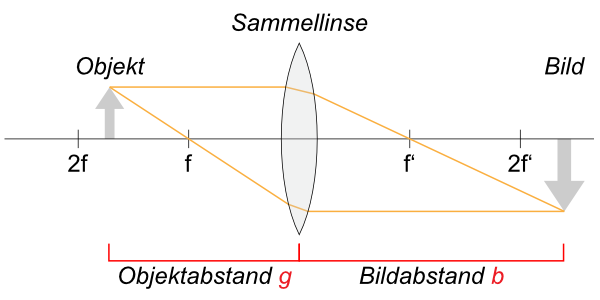
\includegraphics[width=0.49\textwidth]{LinseStrahlengang}}
   \hfill
   \subfigure[Lupe\label{fig:lupestrahl}]
   {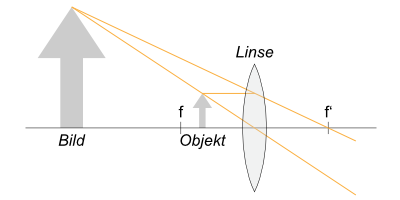
\includegraphics[width=0.49\textwidth]{LupeStrahlengang}}
   \caption{Schematische Strahlengänge von Sammellinse und Lupe jeweils aus \protect\cite[6.3.15, 13 Uhr]{lp18}}
   \label{fig:strahl}
 \end{figure}
Eine Linse ist das wohl wichtigste optische Bauteil.
Sie besteht aus einem speziell geschliffenen Glas, dessen Seiten jeweils entweder konvex oder konkav sind.
Generell kann man Linsen in zwei Gruppen einteilen:
\begin{itemize}
\item \emph{Sammellinsen}, welche zwei konvexe Oberflächen haben und parallel einfallendes Licht auf einen Fukuspunkt (hinter der Linse) bündeln, wie in Abb. \ref{fig:linsestrahl} zu sehen ist, und
\item \emph{Streulinsen}, welche mit zwei konkaven Oberflächen versehen sind und das parallele Licht so streuen, als ob es von dem Brennpunkt (hier vor der Linse) ausgehen würde.
\end{itemize}
Natürlich gibt es auch andere, wie plankonvexe oder konvex-konkave Linsen.
Die Vergrößerung eines Gegenstandes ist definiert als 
\begin{align}
m=\frac{b}{g}=\frac{B}{G}\qquad .\label{eq:vergr}
\end{align}
Hierbei bezeichnet $b$ die Bildweite, $g$ die Gegenstandsweite, $B$ die Bildgröße und $G$ die Gegenstandsgröße.
Allerdings ist das Auge am entspanntesten, wenn sich der Gegenstand in der Brennebene befindet, wodurch $B\approx\infty \si\metre$ wird.
Eine andere sinnvolle Definition der Vergrößerung ist die Winkelvergrößerung.
Sie ist für eine Lupe nach \cite[S.362]{demtroeder2} als
\begin{align}
V=\frac{\varepsilon_\text{mit}}{\varepsilon_\text{ohne}}=\frac{G}{f}\cdot\frac{s_0}{G}=\frac{s_0}{f}\label{eq:winkelvergr}
\end{align}
definiert.
Hierbei ist $f$ die Brennweite der Linse und $s_0\approx 25\si{\centi\meter}$ die Entfernung, in der ein Mensch gerade noch scharf sehen kann.

\subsection{Das Mikroskop}
\begin{figure}[!h]
\centering
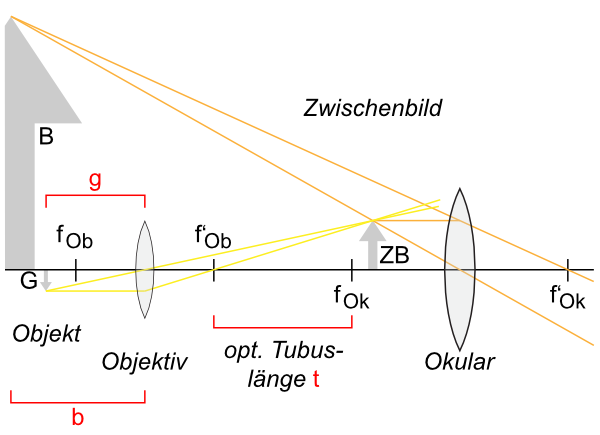
\includegraphics{MikroskopStrahlengang.png}
\caption{Strahlengang des Mikroskops aus \protect\cite[6.3.15, 13 Uhr]{lp18}}
\label{fig:microstrahl}
\end{figure}

Ein Mikroskop besteht aus zwei Sammellinsen, wobei die erste wie ein Teleskop ein reelles Zwischenbild erzeugt (s. Grafik \ref{fig:microstrahl}), welches dann von der zweiten wie mit einer Lupe vergrößert wird.
Die Vergrößerung, welche von einem Mikroskop erzeugt wird, ist daraus resultierend das Produkt der einzelnen Vergrößerungen.
Die Vergrößerung des Okulars ist die einer Lupe, wie in \eqref{eq:winkelvergr}:
\begin{align}
V_\text{Ok}=\frac{s_0}{f_\text{Ok}}\qquad ,
\end{align}
und die des Okulars
\begin{align}
V_\text{Obj}=\frac{b}{g}\qquad .
\end{align}
Da das Objekt ungefähr in der Brennebene liegt, befindet sich das Zwischenbild am Ende des Tubus:
\begin{align}
\notag g\approx -f_\text{Obj} \qquad \text{und}\qquad b\approx t\\
\Rightarrow V_\text{Obj}=-\frac{t}{f_\text{Obj}}\qquad .
\end{align}

Die Gesamtvergrößerung beträgt also
\begin{align}
V=-\frac{t\cdot s_0}{f_\text{Obj}\cdot f_\text{Ok}}\qquad .
\end{align}
Das negative Vorzeichen besagt, dass das Bild auf dem Kopf steht.

\subsection{Auflösungsvermögen}
Werden die zu beobachteten Objekte kleiner, so kann man nicht mehr mit Strahlenoptik rechnen, da diese als Näherung der \textsc{Maxwell}-Gleichungen zu ungenau werden.
Stattdessen muss man die Beugung mit einberechnen.
Sie besagt, dass bei jeder Abbildung Fehler entstehen, so dass ein Punkt nicht in einen Punkt abgebildet werden kann, sondern "`verschmiert"' wird.
Zwei dicht beieinanderliegende Punkte werden so unter Umständen in einen großen "`Klecks"' abgebildet, aus dem man nicht erkennen kann, ob er aus einem oder zwei Objekten besteht.
Das \textsc{Rayleigh}-Kriterium bestimmt, ob diese noch trennbar sind.
Dies wäre der Fall, falls das Hauptmaximum des ersten Bildes mindestens so weit entfernt ist vom Hauptmaximum des zweiten Bildes, wie dessen erstes Minimum.
Die kleinste Winkelauflösung beträgt daher nach \cite[S. 368]{demtroeder2}:
\begin{align*}
	x_\text{min}=1.22\frac{\lambda\cdot f}{D}
\end{align*}
mit der Apertur $D$ (einer charakteristischen Größe des optischen Systems, wie z.B. Durchmesser der Linse) und der Wellenlänge $\lambda$ des beobachten Lichts.
Der beobachtete Öffnungswinkel beträgt $2\sin\alpha=\frac Df$.
Daraus ergibt sich
\begin{align}
x_\text{min}=1.22\frac{\lambda}{2n\cdot\sin\alpha}\approx\frac{\lambda}{N}
\end{align}
mit der numerischen Apertur $N=n\sin\alpha$.



\section{Durchführung}
\label{sec:durchfuehrung}
Der Versuch besteht aus zwei Teilen.
\subsection{Teil A}
Im ersten wird ein Motic-Mikroskop vermessen, wobei jeder Schritt drei mal wiederholt wird.
Zunächst wird die Gesamtvergrößerung bestimmt, in dem das Objektmikrometer auf dem Objekttisch befestigt und das Mikroskop darauf fokussiert wird.
Der Vergleichsmaßstab, welcher auf der Höhe des Objekttisches parallel zu dem Objektmikrometer steht, wird nun mit dem Auge welches nicht durch das Okular guckt beobachtet.
Diese Bilder kommen zur Überlagerung und so kann die Größe der Markierungen bestimmt werden.
Falls hierbei Probleme entstehen muss man zunächst mit dem Auge durch das Okular gucken, bis man etwas sieht.
Danach kann man blinzeln und die Augen entspannt lassen.
Bei der Wiederholung der Versuche ist natürlich immer darauf zu achten, dass sie erneut richtig fokussiert werden.


Anschließend wird das Bild durch den Tubus mit dem Objektiv scharf eingestellt und die zweite Öffnung mit einem Objektiv mit verschiebbarem Mattscheibenokular bestückt.
Diese wird nun (bei verdunkeltem Raum) so verschoben, dass das Zwischenbild scharf auf ihr zu erkennen ist.
Dann wird mit einem Messschieber die Größe des abgebildeten Zwischenbildes bestimmt.
Dieses wird ebenfalls dreifach je für das 10-fache und das 40-fache Okular wiederholt, wobei der Objekttisch stets auf der selben Höhe bleibt.

\subsection{Teil B}
\begin{figure}[h]
\centering
\def\svgwidth{0.7\linewidth}
\input{schieneStrahlengang.pdf_tex}
\caption{Aufbau zur Bestimmung der Blendenweite, bei der die Linien ununterscheidbar werden\protect\footnotemark}
\label{fig:aufbau2}
\end{figure}
\footnotetext{nach \url{http://genug-davon.de/img/aprakt/v18/schieneStrahlengang.tar}}
Der zweite Teil verwendet den Aufbau aus Abb. \ref{fig:aufbau2}.
Hierbei wird vor der Lampe mit dem Rotlichtfilter der Glasmaßstab so aufgestellt, dass dieser scharf durch das Objektiv abgebildet wird.
Dann wird zwischen Objektiv und Glasscheibe ein Einfachspalt gestellt, dessen Breite variabel einstellbar ist.
Wird dieser immer mehr geschlossen, so wird das Bild erkennbar unschärfer.
Es ist nun die Öffnung des Spaltes zu suchen, bei der gerade so die kleinen Skalenteile nichtmehr unterscheidbar sind.
Dies erfordert etwas Übung, da der Punkt gesucht wird, bei dem die komplette Skala zu einem Grauschleier wird.
Nun wird die Entfernung zwischen Glasmaßstab und Einfachspalt gemessen.

Anschließend muss die Breite des Spaltes bestimmt werden.
Hierfür nimmt man den Maßstab aus der Schiene und bewegt den Schpalt so weit vom Okular fort, dass dieser scharf erkennbar ist.
Dann wird der eine Rand des Spaltes durch das Objektiv mit dem Millimetergewinde fixiert und die Position notiert.
Selbiges wird mit dem anderen Rand getan, so dass die Differenz den Durchmesser ergibt.

Nun wird der Spalt wieder aus dem Strahlengang entfernt und erneut durch den Plexiglasstab ersetzt.
Und der Stab wird auf eine Position verschoben, in der die Vorderseite (ohne die Gitterlinien) scharf erkennbar ist.
Auch das Okular wird jetzt durch eine Lochblende ausgetauscht, so dass der Strahlengang wie in Abb. \ref{fig:strahl3} ist.
Sie sitzt ungefähr in der Ebene des Zwischenbildes, so dass durch sie die Spalte am anderen Plexiglasende zu erkennen sind.
Deren sichtbare Anzahl ist nun zu notieren, ebenso wie die Länge des Stabes.

\begin{figure}[h]
\centering
\def\svgwidth{0.7\linewidth}
\input{strahlengang3.pdf_tex}
\caption{Aufbau zur optischen Schiene mit dem Plexiglasstab\protect\footnotemark}
\label{fig:strahl3}
\end{figure}
\footnotetext{nach \url{http://genug-davon.de/img/aprakt/v18/strahlengang3.tar}}

\section{Auswertung}
\label{sec:auswertung}
\subsection{Teil A}
Um die Vergrößerung von Mikroskop und Objektiv zu berechnen, wird Formel \eqref{eq:vergr} verwendet.
Die Werte der kleinen Skala wurden als richtig angenommen und dafür diejenigen der großen Skala mit einem größeren Fehler versehen.
Daraus ergibt sich mit der Gaußschen Fehlerfortpflanzung:
\begin{align*}
\sigma_V=\frac{\sigma_B}{G}
\end{align*}
mit $B=\frac{\text{Skalenteile}}{\frac{20\text{Skalenteile}}{1\si{\centi\metre}}}$.
Die sich ergebenden Werte aus Tabelle \ref{tab:vergr} sind die gewichteten Mittelwerte.
\begin{table}[!h]
\centering
\begin{tabular}{|c||c|c|c|}
\hline
 & $V$ & $V_\text{Obj}$ & $V_\text{Ok}=\frac{V}{V_\text{Obj}}$\\\hline\hline
10-fach & $98.4\pm0.7$ & $9.44\pm0.07$ & $10.4\pm 0.1$ \\\hline
40-fach & $365\pm 3$ & $40.8\pm 0.3$ &$8.95\pm0.09$ \\\hline
\end{tabular}
\caption{Die Vergrößerungen des Mikroskops aus den gewichteten Mittelwerten der Messungen}
\label{tab:vergr}
\end{table}


Die Vergrößerung des Okulars ergibt sich aus
\begin{align}
V_\text{Ok}&=\frac{V}{V_\text{Obj}}\qquad \text{mit}\\
\sigma_{V_\text{Ok}}&=\sqrt{\left(\frac{\sigma_V}{V_\text{Obj}}\right)^2+\left(\sigma_{V_\text{Obj}} \frac{V}{V_\text{Obj}^2} \right)^2}
\end{align}
und der gewichtete Mittelwert aus Tabelle \ref{tab:vergr} ergibt:
\begin{align}
V_\text{Ok}=9.60\pm0.07\qquad .
\end{align}

%begin{table}
%centering
%begin{tabular}{|c|c|c|c|c|c|c|c|}
%
% 100, 2 $	&$408,8$	&$ 97.0, 2 $	&$ 368, 8 $	&$ 8.6, 0.2 $	&$ 35.2, 0.8 $	&$ 12.9, 0.2 $	&$ 52.8, 0.8 $	\\
% 101, 3 $	&$412,8$	&$ 95, 2 $	&$ 348, 5 $	&$ 8.6, 0.2 $	&$ 34.9, 0.5 $	&$ 13.5, 0.3 $	&$ 52.0, 0.7 $	\\
% 102, 2 $	&($310,10$)	&$ 100, 2 $	&$ 360, 10 $	&$ 8.4, 0.1 $	&$ 35.2, 0.8 $	&$ 13.4, 0.4 $	&$ 54, 2 $	\\
%       	&	&$ 95, 2 $	&$ 351, 5 $	&		&		&		&		\\
%
%
%
%end{tabular}
%caption{Messwerte aus Teil A}
%label{tab:MesswerteA}
%end{table}

Die Brennweite der Linse berechnet sich durch
\begin{align}
f&=\frac{\Delta t}{V_\text{m. Tub} - V_\text{o. Tub}}\\
\sigma_f&=\frac{1}{\left(V_\text{o. Tub} - V_\text{m. Tub}\right)^{2}} \sqrt{\sigma_{\Delta t}^{2} \left(V_\text{o. Tub} - V_\text{m. Tub}\right)^{2} + \Delta t^{2} \left(\sigma_{V_\text{o. Tub}}^{2} + \sigma_{V_\text{m. Tub}}^{2}\right)}
\end{align}
und es ergeben sich für die Brennweiten aus den gewichteten Mittelwerten
\begin{align}
f_\text{10x}=(0.0182 \pm 0.0007)\si\metre\\
f_\text{40x}=(0.0048 \pm 0.0002)\si\metre
\end{align}

\subsection{Teil B}
Laut der Praktikumsanleitung haben die Linien auf dem Plexiglasstab einen Abstand $x_\text{min}=0.1\si{\milli\metre}$.
Können diese in einem Abstand $e=(0.0276\pm0.0001)\si{\metre}$ von dem Mikroskop nicht mehr voneinander unterschieden werden, so beträgt das Auflösungsvermögen gerade $A=\frac{e}{x_\text{min}}=276\pm2$.

Die Spaltbreite betrug $r=(0.388\pm0.001)\si{\milli\metre}$.
Der vorhandene Öffnungswinkel betrug somit
\begin{align*}
\sin\varphi=\frac{r}{e}=0.01406 \pm 0.00006
\end{align*}
Die Wellenlänge betrug $650\si{\nano\metre}$ und somit ergibt sich
\begin{align*}
A=\frac{e\cdot n\sin\varphi}{\lambda}=\frac{r}{\lambda}=597 \pm 2
\end{align*}

In Abb. \ref{fig:strahl3} ist der Strahlengang zu sehen.
Im Dreieck innerhalb des Plexiglases gilt nach dem Satz des Pythagoras
\begin{align}
\sin\alpha&=\frac{d/2}{\sqrt{d^2/4+L^2}}\\
\Rightarrow N&=n\sin\alpha=n\frac{d/2}{\sqrt{d^2/4+L^2}}
\end{align}
mit der Länge $L$ des Stabes und dem Brechungsindex $n\approx1.49$ in seinem Inneren.
Die Dicke $d$ wurde aus der Anzahl der beobachteten Striche im Inneren berechnet.
Es waren 10 komplett zu sehen, so dass die Breite $d\approx 5\si{\milli\metre}$ betrug.
\begin{align*}
\Rightarrow N=0.090
\end{align*}

\section{Diskussion}
\label{sec:diskussion}
\subsection{Teil A}
Bei der Messung des 40-fachen Objektives wurde offensichtlich ein Messwert falsch aufgezeichnet.
Es ergeben sich Vergrößerungen von 408, 412 und 310.
Augenscheinlich wurde bei einer kleinen Skala von 4 Skalenteilen statt $8.2\si{\centi\metre}$ der Wert $6.2\si{\centi\metre}$ aufgeschrieben.
Ansonsten ergäbe der letzte Wert eine 410-fache Vergrößerung, welche wesentlich plausiebler ist.

In Tabelle \ref{tab:vergr} ist zu erkennen, dass die Vergrößerung des Okulars $V_\text{Ok}$ bei den Messungen mit 10- und 40-facher Vergrößerung des Objektivs stark voneinander abweicht.
Das Okular hat laut Beschriftung eine Vergrößerung um den Faktor 10, so dass beide Werte ihn nicht in ihrem Fehlerintervall einschließen.
Die Abweichungen lassen sich auch dadurch erklären, dass der scharfe Punkt insbesondere des langen Tubuses nicht genau zu erkennen war.
Wir haben ihn vermutlich zu weit hineingeschoben, so dass die Vergrößerung zu klein war.
Der gewichtete Mittelwert der Vergrößerung des Objektives mit $9.60\pm0.07$ ist jedoch nur um 4\% kleiner als laut Beschriftung, so dass diese Messung dennoch als Erfolg zu sehen ist.

Die Brennweiten der beiden Objektive besitzen nur ein 4\% des Wertes großes Fehlerintervall, was angemessen erscheint.
Es ist allerdings nur ein Faktor 3.79 zwischen den beiden, statt dem erwarteten 4.


\subsection{Teil B}
Der zweite Teil der Versuchsdurchführung lässt mehr Interpretationsspielraum.

Die Bestimmung der Breite des Spaltes war insofern herausfordernd, als dass das Gehäuse schräg war, wodurch nur eine Seite des Spaltes scharfzustellen war.
Des weiteren hatte unser Objektiv kein Fadenkreuz, so dass wir ein Staubkorn darin als Fixpunkt nehmen mussten.
Dies ist natürlich wesentlich ungenauer, so dass die Bestimmung der Spaltbreite vermutlich ein zu geringes Fehlerintervall aufweist.

Das Auflösevermögen, welches theoretisch bestimmt ist durch $A=\frac{r}{\lambda}=597\pm2$ ist mehr als doppelt so groß, wie das durch $A=\frac{e}{x_\text{min}}=276\pm2$ bestimmte.
Dies lässt sich insofern erklären, als dass vermutlich die Striche noch zu unterscheiden gewesen sind, jedoch nur verschwommen und so falsche Annahmen gemacht wurden.





\bibliography{literatur}
\bibliographystyle{babalpha}
\end{document}
